\subsection*{Экспериментальная установка}


Свет от источника $S$ с помощью линзы фокусируется на входную щель призменного монохроматора УМ-2, выделяющего узкий спектральный интервал, и попадает на катод фотоэлемента ФЭ.
\begin{figure}[h]
    \centering
    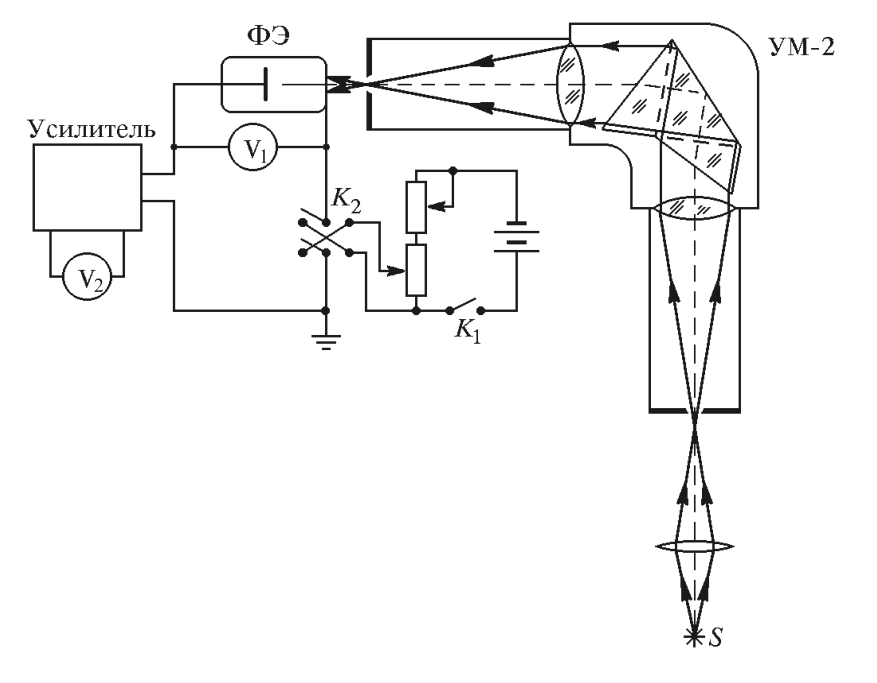
\includegraphics[width=0.5\textwidth]{imgs/exp.png}
    \caption{Схема экспериментальной установки}
    \label{fig:exp}
\end{figure}
Фотоэлемент представляет собой откаченный до высокого вакуума стеклянный баллон, внутри которого расположены два электрода: фотокатод и анод. Фотоэлемент обладает спектральной чувствительностью в области длин волн от $300$ до $850$ нм, наибольшая чувствительность ФЭ в области от $400$ до $500$ нм. 

Фототок, протекающий в ФЭ, мал, так что для его измерения используется усилитель постоянного тока. Тормозящий потенциал регулируется, измерения осуществляются с помощью цифрового вольтметра.




\subsection*{Измерения}

Для начала измерим 
